\documentclass[11pt,a4paper]{article}

% =============================================
% Packages
% =============================================
\usepackage[utf8]{inputenc}
\usepackage[T1]{fontenc}
\usepackage{amsmath,amssymb,amsthm}
\usepackage{graphicx}
\usepackage{booktabs}
\usepackage{enumitem}
\usepackage{geometry}
\usepackage{setspace}
\usepackage{hyperref}
\usepackage[numbers]{natbib}
\usepackage{xcolor}
\usepackage{fancyhdr}
\usepackage{titlesec}
\usepackage{float}
\usepackage{caption}
\usepackage{tcolorbox}
\usepackage{tabularx}
\usepackage{array}
\usepackage{url}
\urlstyle{tt}

% Public repository (GitHub; Zenodo DOI filled at archival release)
\newcommand{\ExcessThreeRepo}{https://github.com/johelpadilla/excess3}
\newcommand{\ExcessThreeRepoShort}{github.com/johelpadilla/excess3}
% \newcommand{\ExcessThreeDOI}{10.5281/zenodo.XXXXXXX}  % set at Zenodo release

\geometry{margin=1in}
\onehalfspacing

\titleformat{\section}{\large\bfseries}{\thesection}{0.6em}{}
\titleformat{\subsection}{\normalsize\bfseries}{\thesubsection}{0.5em}{}
\titleformat{\subsubsection}{\normalsize\itshape}{\thesubsubsection}{0.5em}{}

\pagestyle{fancy}
\fancyhf{}
\fancyhead[L]{\small excess$^3$ in the Systemic Tau / RECD paradigm}
\fancyhead[R]{\small \thepage}
\renewcommand{\headrulewidth}{0.4pt}

\hypersetup{
  colorlinks=true,
  linkcolor=blue!60!black,
  citecolor=blue!60!black,
  urlcolor=blue!70!black,
  pdftitle={excess3: A Pre-Specified Continuous Proxy for Order-3 Synergistic Surplus},
  pdfauthor={Johel Padilla-Villanueva},
  pdfkeywords={excess3, RECD, Systemic Tau, synergistic information, PID, ordinal patterns}
}

% Macros for validation numbers (filled after synthetic run)
% Auto-generated by scripts/fill_numbers_from_json.py — do not edit by hand
\newcommand{\NumT}{1000}
\newcommand{\NumEvent}{500}
\newcommand{\NumR}{25}
\newcommand{\NumB}{99}

% G0
\newcommand{\GzeroPre}{1.8331}
\newcommand{\GzeroPost}{1.8358}
\newcommand{\GzeroDelta}{+0.0028}
\newcommand{\GzeroMedP}{0.560}
\newcommand{\GzeroFrac}{4\%}
\newcommand{\GzeroOccPost}{1.000}

% G1
\newcommand{\GonePre}{1.8308}
\newcommand{\GonePost}{1.7332}
\newcommand{\GoneDelta}{-0.0977}
\newcommand{\GoneMedP}{0.010}
\newcommand{\GoneFrac}{92\%}
\newcommand{\GoneOccPost}{1.000}

% G2
\newcommand{\GtwoPre}{1.6273}
\newcommand{\GtwoPost}{1.6192}
\newcommand{\GtwoDelta}{-0.0081}
\newcommand{\GtwoMedP}{0.510}
\newcommand{\GtwoFrac}{8\%}
\newcommand{\GtwoOccPost}{1.000}

% G3
\newcommand{\GthreePre}{1.8374}
\newcommand{\GthreePost}{1.7893}
\newcommand{\GthreeDelta}{-0.0482}
\newcommand{\GthreeMedP}{0.080}
\newcommand{\GthreeFrac}{40\%}
\newcommand{\GthreeOccPost}{1.000}



\title{\textbf{excess$^3$: A Pre-Specified Continuous Proxy for\\
Order-3 Synergistic Surplus in the Systemic Tau / RECD paradigm}\\[0.4em]
\large Methods, Null Models, and Synthetic Validation}

\author{
Johel Padilla-Villanueva \\
\textit{Department of Environmental Health, University of Puerto Rico} \\
ORCID: \href{https://orcid.org/0000-0002-5797-6931}{0000-0002-5797-6931} \\
\texttt{johelpadilla@gmail.com} \\
\texttt{joel.padilla2@upr.edu}
}

\date{Preprint v1.0 \quad | \quad July 2026 \\[0.25em]\small Repository: \href{\ExcessThreeRepo}{\ExcessThreeRepoShort}}

\begin{document}
\maketitle

% =============================================
\begin{abstract}
High-order multivariate dependence (structure that cannot be reduced to
pairwise interactions) is central to theories of integration, emergence,
and critical reorganisation, yet it is difficult to estimate and easy to
over-interpret. Within the Systemic Tau / Discrete Extramental Clock
(RECD) paradigm, Level~3 of the nested ordinal hierarchy is intended to
capture exactly this irreducible joint surplus. Here we provide a
canonical, honest specification of its continuous operational form,
\textbf{excess$^{3}$} (denoted \texttt{excess3} in code and software).

excess$^3$ is a hybrid of (i)~synergistic excess of total correlation over a
pairwise mutual-information baseline ($\mathrm{Syn}$) and (ii)~weighted
log-ratio surprise of joint symbol tuples under a full independence model
($\mathrm{Surp}$), combined with fixed a~priori weights
$0.6/0.4$. Continuous excess$^3$ is the primary Level-3 readout;
the binary indicator
$\Phi_3=\mathbf{1}\{\mathrm{excess3}>\theta_3\}$ is retained only for discrete
tick counts. We argue that the weights must not be optimised on the
scientific dataset if falsifiability is to be preserved; that inference
should use phase-shuffle surrogates on the \emph{full} statistic
(e.g.\ $\Delta\mathrm{excess3}$), not mean-versus-mean alone; that nesting of
$\Phi_1,\Phi_2,\Phi_3$ is operational and parallel rather than a hard logical
implication; and that excess$^3$ measures high-order statistical dependence,
not causation, and is a computable proxy rather than a full partial
information decomposition (PID) atom.

We validate the construction on four synthetic arms: independent AR(1)
channels (near-null), a shared-latent coupling jump (planted joint
reorganisation), coupled logistic maps, and a pure pairwise control
($R=\NumR$ realisations, $B=\NumB$ phase-shuffle surrogates, $T=\NumT$).
Under reference hyperparameters, phase-shuffle tests on
$|\Delta\mathrm{excess3}|$ behave as predicted for null vs.\ planted
structure: the near-null arm (G0) has mean $\Delta=\GzeroDelta$ and median
$p=\GzeroMedP$ ($\GzeroFrac$ of realisations with $p<0.05$), while planted
shared-latent reorganisation (G1) yields mean $\Delta=\GoneDelta$, median
$p=\GoneMedP$, and $\GoneFrac$ extreme realisations (two-sided; the sign is
negative under this generator because stronger common coupling inflates
pairwise baselines relative to residual multiinformation). The logistic arm
(G2) is near-null in this design (mean $\Delta=\GtwoDelta$); the pairwise
control (G3) is intermediate (mean $\Delta=\GthreeDelta$, median
$p=\GthreeMedP$). At the reference binary threshold $\theta_3=0.08$,
$\Phi_3$ occupancy saturates on these generators because continuous
excess$^3$ lives near $O(1)$; discrimination resides in continuous $\Delta$.
We close with estimation caveats, downstream uses, the path to excess$^k$,
and explicit limitations. Scope is directional synthetic validation under a
pre-specified protocol---not a multi-domain empirical atlas---so that later
applied papers can cite a frozen Level-3 contract rather than re-derive ad~hoc
variants.
\end{abstract}

\noindent\textbf{Keywords:}
excess$^3$, synergistic information, partial information decomposition,
RECD, Systemic Tau, ordinal patterns, total correlation, surrogate testing,
complex systems, multivariate dependence

\vspace{0.4cm}

% =============================================
\section{Introduction}
\label{sec:intro}

Complex systems often reorganise not only in the amplitude of individual
observables but in the \emph{joint} structure that binds them. Classical
early-warning signals based on variance and lag-1 autocorrelation remain
powerful for a class of local bifurcations \citep{Scheffer2009,Dakos2012}, yet
they are primarily univariate and magnitude-driven. Relational and ordinal
tools---Kendall concordance, Bandt--Pompe symbolic dynamics, transfer
entropy, and partial information decomposition---shift attention from size
of fluctuations to organisation among variables
\citep{Kendall1938,BandtPompe2002,Schreiber2000,Williams2010}.

The Systemic Tau / RECD paradigm pairs two complementary constructs
\citep{Padilla2026framework,Padilla2025preprints}. \textbf{Systemic Tau}
($\tau_s$) aggregates multivariate rank concordance into a continuous
thermometer of relational coherence. The \textbf{Discrete Extramental Clock}
(RECD) advances an intrinsic time from hierarchical \emph{ordinal
conjunctions}: coincidence ($\Phi_1$), persistent pairwise relations
($\Phi_2$), and irreducible synergistic surplus (Level~3). The continuous
Level-3 measure is excess$^3$; its thresholded form is $\Phi_3$.

In applied reports, Level~3 is frequently the most misunderstood piece.
Binary $\Phi_3$ may remain near zero under realistic noise while continuous
excess$^3$ still moves; weights $0.6/0.4$ look arbitrary unless
pre-specification is explained; surrogate tests are applied to the wrong
summary; nesting is read as logical implication; and excess$^3$ is mistaken
for a full PID synergy atom or for a causal claim. This paper is the
canonical methods specification dedicated to closing those gaps.

\paragraph{Contributions.}
\begin{enumerate}[leftmargin=*,itemsep=2pt]
  \item A complete formal definition of excess$^3$ aligned with the
  reference software implementation.
  \item An explicit methodological rationale for fixed a~priori weights and
  continuous primacy over $\Phi_3$.
  \item A recommended null protocol (phase-shuffle on the full statistic).
  \item A synthetic validation battery (G0--G3) with pre-specified success
  criteria and sensitivity checks.
  \item An honest map of what excess$^3$ is \emph{not}: causation, full PID,
  proof of strong emergence.
\end{enumerate}

\paragraph{Roadmap.}
Section~\ref{sec:related} situates excess$^3$ among multivariate information
measures (with a comparison table). Section~\ref{sec:definition} gives the
formal construction, a key-definitions box, an intuitive magnitude reading,
and a worked toy window. Section~\ref{sec:boundaries} states boundaries.
Section~\ref{sec:design} consolidates six design decisions that are often
misread in applied reports (weights, Syn vs.\ Surp, continuous primacy,
PID scope, nulls, nesting). Section~\ref{sec:inference} details null
inference. Section~\ref{sec:estimation} discusses estimation practice.
Section~\ref{sec:validation} reports synthetic validation.
Sections~\ref{sec:downstream}--\ref{sec:limitations} cover uses and
limitations; Section~\ref{sec:discussion} discusses outlook and a reporting
checklist.

% =============================================
\section{Related measures}
\label{sec:related}

excess$^3$ lives in a neighbourhood of classical and modern multivariate
information tools, without claiming to replace them.
Table~\ref{tab:compare} positions the proxy relative to the measures
readers most often confuse with it---in particular, how it differs from
PID and O-information.

\begin{table}[H]
\centering
\caption{Positioning of excess$^3$ relative to related multivariate
interdependence measures.}
\label{tab:compare}
\small
\begin{tabularx}{\textwidth}{@{}>{\raggedright\arraybackslash}p{2.6cm}
  >{\raggedright\arraybackslash}X
  >{\raggedright\arraybackslash}p{1.6cm}
  >{\raggedright\arraybackslash}X@{}}
\toprule
\textbf{Measure} & \textbf{Captures mainly} & \textbf{Cost} &
\textbf{Relation to excess$^3$} \\
\midrule
Interaction information
  $I(X;Y;Z)$
  & Synergy $+$ redundancy (can be negative)
  & Low
  & Partially related; excess$^3$ targets a non-negative residual
    surplus rather than a signed triple interaction. \\
O-information /
  S-information
  & Global redundancy vs.\ synergy decomposition
  & Medium
  & More global; not locked to order exactly~3. \\
PID synergy atom
  & Pure synergistic atom of the PID lattice
  & High
  & Conceptual target. excess$^3$ is a \textbf{computable proxy}
    when a stable PID estimator is not feasible. \\
\textbf{excess$^3$}
  (this work)
  & Hybrid order-3 synergistic surplus
  & Low--med.
  & Pre-specified continuous proxy with fixed $0.6/0.4$ weights. \\
\bottomrule
\end{tabularx}
\end{table}

\paragraph{Brief notes.}
Watanabe's total correlation (multiinformation)
$\mathrm{TC}=\sum_i H(X_i)-H(X_{1:N})$
\citep{Watanabe1960,McGill1954} is the backbone of the $\mathrm{Syn}$ term.
Averaged pairwise MI supplies the order-2 baseline that $\mathrm{Syn}$
subtracts. The three-variable interaction information $I(X;Y;Z)$ can be
negative, a classical synergy signature
\citep{McGill1954,Timme2018}; excess$^3$ aims at a related residual but is
not identical to $I(X;Y;Z)$. O-/S-information separate redundancy-like and
synergy-like modes globally \citep{Rosas2019}. PID lattices isolate unique,
redundant, and synergistic atoms
\citep{Williams2010,Bertschinger2014,Finn2018,Lizier2014}; the synergistic
atom is the conceptual target of Level~3, while excess$^3$ remains a
\emph{pre-specified computable proxy}. Directed information flow
\citep{Schreiber2000} is complementary; lagged excess$^3$ is future work.

% =============================================
\section{Formal definition}
\label{sec:definition}

\begin{tcolorbox}[
  colback=blue!5!white,
  colframe=blue!75!black,
  title={\textbf{Key definitions for excess$^3$}},
  fonttitle=\bfseries,
  boxrule=0.8pt,
  left=4pt,right=4pt,top=2pt,bottom=2pt,
  label=box:keydefs
]
\begin{description}[leftmargin=2.2em,itemsep=3pt,parsep=0pt,topsep=2pt]
  \item[TC (Total Correlation)]
    Total shared information among the $N$ variables
    (Watanabe--McGill multiinformation). Backbone of the $\mathrm{Syn}$ term.
  \item[$I_{\mathrm{pair}}$]
    Order-2 baseline: mean pairwise mutual information scaled so that it is
    comparable to TC.
  \item[Syn]
    Synergistic residual:
    $\mathrm{Syn}=[\mathrm{TC}-I_{\mathrm{pair}}]_+$.
    What remains after subtracting pairwise interactions.
  \item[Surp]
    Independence surprise: how much more often joint tuples occur than
    expected under full independence $P(X)P(Y)P(Z)$ (product of marginals).
  \item[excess$^3$]
    Hybrid order-3 synergistic-surplus proxy:
    $\mathrm{excess3}=0.6\,\mathrm{Syn}+0.4\,\mathrm{Surp}$.
    Weights are fixed a~priori.
  \item[$\Phi_3$]
    Binary tick $\mathbf{1}\{\mathrm{excess3}>\theta_3\}$---secondary
    discretisation only; continuous excess$^3$ is primary.
\end{description}
\end{tcolorbox}

\subsection{Symbolic substrate}
\label{sec:symbols}

Let $X_t\in\mathbb{R}^N$ be a multivariate series. Each coordinate is
encoded by Bandt--Pompe ordinal patterns of embedding dimension $m$ and
delay $\tau$ \citep{BandtPompe2002,Amigo2010}, yielding a symbol matrix
$S_t\in\{0,\ldots,m!-1\}^N$ for $t=1,\ldots,T_{\mathrm{eff}}$. All Level-3
quantities are estimated on a sliding window of length $w$ ending at $t$,
denoted $S_{[t-w+1,t]}$.

\subsection{Total correlation and pairwise baseline}
\label{sec:tc}

Write $\pi^{(i)}$ for the $i$-th coordinate of the windowed symbols and
$H(\cdot)$ for plug-in Shannon entropy in bits. Total correlation on the
window is
\begin{equation}
\label{eq:tc}
\mathrm{TC}(t)
=\sum_{i=1}^{N} H\bigl(\pi^{(i)}\bigr)
-H\bigl(\pi^{(1)},\ldots,\pi^{(N)}\bigr).
\end{equation}
A pairwise baseline scales the mean pairwise mutual information so that it
is dimensionally comparable to a multiinformation residual
\citep{Padilla2026framework}:
\begin{equation}
\label{eq:ipair}
I_{\mathrm{pair}}(t)
=(N-1)\cdot
\frac{2}{N(N-1)}
\sum_{1\le i<j\le N}
I\bigl(\pi^{(i)};\pi^{(j)}\bigr)
=(N-1)\,\overline{I}_{ij}(t).
\end{equation}

\subsection{Synergy residual and independence surprise}
\label{sec:syn_surp}

\begin{equation}
\label{eq:syn}
\mathrm{Syn}(t)
=\bigl[\mathrm{TC}(t)-I_{\mathrm{pair}}(t)\bigr]_+ ,
\end{equation}
where $[\cdot]_+=\max\{\cdot,0\}$. $\mathrm{Syn}$ subtracts order-2 structure
so that residual multiinformation is emphasised.

Independence surprise contrasts the empirical joint frequency
$p_{\mathrm{obs}}(s)$ of each joint symbol $s$ with the product of marginals
$p_{\mathrm{ind}}(s)=\prod_{i=1}^{N}p_i(s_i)$:
\begin{equation}
\label{eq:surp}
\mathrm{Surp}(t)
=\sum_{s} p_{\mathrm{obs}}(s)\,
\bigl[\log_2 p_{\mathrm{obs}}(s)-\log_2 p_{\mathrm{ind}}(s)\bigr]_+ .
\end{equation}
$\mathrm{Surp}$ detects joint configurations that occur more often than under
complete independence---tuples over-represented relative to the product of
marginals. The two terms are complementary: $\mathrm{Syn}$ controls a
pairwise MI baseline inside the multiinformation geometry (it
\emph{subtracts} order-2 structure); $\mathrm{Surp}$ scores co-occurrence
against full factorisation. Their joint role is restated among the six
design decisions of Section~\ref{sec:design}.

\subsection{Hybrid excess$^3$ and binary $\Phi_3$}
\label{sec:hybrid}

\begin{equation}
\label{eq:excess3}
\mathrm{excess3}(t)
=0.6\,\mathrm{Syn}(t)+0.4\,\mathrm{Surp}(t).
\end{equation}
The weights $(0.6,0.4)$ are \textbf{heuristic constants fixed a~priori}
from controlled simulations \emph{before} analysing scientific target
datasets. They are not tuned by cross-validation or grid search on the
dataset of interest. That choice is part of the methodological design of
the paradigm: if weights are optimised on the same records used for
scientific claims, excess$^3$ ceases to be a pre-specified test statistic
and becomes a post-hoc descriptor vulnerable to overfitting.

The binary Level-3 event indicator is
\begin{equation}
\label{eq:phi3}
\Phi_3(t)=\mathbf{1}\bigl\{\mathrm{excess3}(t)>\theta_3\bigr\},
\end{equation}
with threshold $\theta_3>0$ (reference values $\theta_3\in\{0.08,0.10\}$ in
software defaults). Continuous excess$^3$ is the \textbf{primary} readout
for magnitude, gradients, and contrasts. $\Phi_3$ is a
\textbf{secondary discretisation} for tick counts, raster-like displays,
and rate analyses. Reporting only ``$\Phi_3$ never fired'' without
continuous curves is methodologically incomplete under noise
\citep{Padilla2026framework}.

\paragraph{Interpretation of magnitudes.}
Values of $\mathrm{excess3}(t)$ near zero indicate that the joint structure of
the three (or $N$) variables is largely explainable by pairwise interactions
or by independence under the plug-in window estimator.
Consistently positive values away from zero
(typically $\gtrsim 0.10$--$0.20$ depending on domain and entropy scale;
\emph{not} a universal cut-off) suggest detectable order-3 synergistic
surplus.
In practice, the contrast $\Delta\mathrm{excess3}$ (pre/post or between
conditions) is usually more informative than the absolute level.
Note that $\Delta\mathrm{excess3}$ can be \emph{negative} even under strong
joint reorganisation if increased common coupling inflates the pairwise
baseline more than the multiinformational residual---as observed in the G1
synthetic arm (Section~\ref{sec:validation}).
Absolute scales also shift with $m$, $w$, alphabet size, and $N$; always
interpret with a null (Section~\ref{sec:inference}) rather than a floating
global threshold.

\subsection{Toy numerical example}
\label{sec:toy}

To make the algebra concrete, consider a single window of length $w=8$ with
$N=3$ already-encoded ordinal symbols (alphabet $\{0,1\}$). The eight joint
rows implement a classical XOR-like lock---each pair of coordinates is
independent, but the triple is fully determined:
\begin{equation*}
\begin{array}{c@{\;}c@{\;}c}
\pi^{(1)} & \pi^{(2)} & \pi^{(3)} \\
\hline
0 & 0 & 0 \\
0 & 1 & 1 \\
1 & 0 & 1 \\
1 & 1 & 0 \\
0 & 0 & 0 \\
0 & 1 & 1 \\
1 & 0 & 1 \\
1 & 1 & 0
\end{array}
\qquad
\begin{array}{l}
\text{(each of the four distinct joint tuples}\\
\text{appears twice: }p_{\mathrm{obs}}=1/4\text{).}
\end{array}
\end{equation*}
Plug-in entropies (bits) give $H(\pi^{(i)})=1$ for each $i$ and
$H(\pi^{(1)},\pi^{(2)},\pi^{(3)})=2$, hence
\begin{equation*}
\mathrm{TC}
=\sum_i H(\pi^{(i)})-H_{\mathrm{joint}}
=3-2=1.
\end{equation*}
Every pairwise MI vanishes ($I(\pi^{(i)};\pi^{(j)})=0$), so
$I_{\mathrm{pair}}=(N-1)\overline{I}_{ij}=0$ and
\begin{equation*}
\mathrm{Syn}=[\mathrm{TC}-I_{\mathrm{pair}}]_+=1.
\end{equation*}
For each joint tuple $s$, the independence product is
$p_{\mathrm{ind}}(s)=(1/2)^3=1/8$, while $p_{\mathrm{obs}}(s)=1/4$, so
$\log_2(p_{\mathrm{obs}}/p_{\mathrm{ind}})=1$ and each of the four types
contributes $(1/4)\cdot 1=0.25$ to surprise:
\begin{equation*}
\mathrm{Surp}=4\times 0.25=1.
\end{equation*}
Therefore
\begin{equation*}
\mathrm{excess3}
=0.6\cdot\mathrm{Syn}+0.4\cdot\mathrm{Surp}
=0.6\cdot 1+0.4\cdot 1=1.0.
\end{equation*}
Both hybrid ingredients fire: $\mathrm{Syn}$ because TC exceeds the
pairwise baseline, and $\mathrm{Surp}$ because joint co-occurrence beats
full factorisation. The same arithmetic is reproduced by the companion
script \path{scripts/toy_example.py} and by the reference
\path{_synergy_and_surprise} routine.

\paragraph{Contrast: pure common driver.}
If instead all three coordinates are identical
(only the joints $(0,0,0)$, $(1,1,1)$, and $(2,2,2)$), pairwise MI
absorbs essentially all of TC under the $I_{\mathrm{pair}}$ scaling, so
$\mathrm{Syn}\to 0$ while $\mathrm{Surp}$ remains large (joint tuples are far
more frequent than under independence). excess$^3$ then lives almost entirely
on the surprise leg. This is intentional: pure redundant locking is not the
same geometry as XOR-like order-3 structure, and the hybrid keeps both modes
visible rather than forcing a single atom.

\subsection{Role in the RECD clock}
\label{sec:recd}

An unweighted RECD increment may combine levels as
\begin{equation}
\label{eq:drecd}
\Delta\mathrm{RECD}_0(t)
=\Phi_1(t)+\Phi_2(t)+\mathrm{excess3}(t),
\end{equation}
or with binary Level~3, $\Phi_1+\Phi_2+\Phi_3$. Weighted RECD replaces
coefficients by regime-dependent $\alpha_\ell(\lambda)$ modulated by a cue
derived from $|\tau_s|$ \citep{Padilla2026framework}. The present paper does
not re-litigate $\lambda$; it fixes the Level-3 building block.

\paragraph{Operative nesting.}
Conceptually one may write $\Phi_3\supset\Phi_2\supset\Phi_1$ to express that
deeper claims are stronger. Operationally, $\Phi_1$, $\Phi_2$, and
excess$^3$/$\Phi_3$ are computed \textbf{in parallel} from $S_t$. There is
\textbf{no hard logical implication}
$\Phi_1\Rightarrow\Phi_2\Rightarrow\Phi_3$ in the reference code.
Irreducibility of order~3 is inferred \emph{statistically} via the excess
construction (Syn$+$Surp after removing pairwise baselines), not by
forcing a chain of Boolean implications.

% =============================================
\section{What excess$^3$ is not}
\label{sec:boundaries}

\begin{enumerate}[leftmargin=*,itemsep=3pt]
  \item \textbf{Not causation.}
  excess$^3$ quantifies high-order statistical dependence
  (co-occurrence beyond pairs). Causal language requires lagged or directed
  variants and/or interventional designs.

  \item \textbf{Not a full PID lattice.}
  It correlates with synergistic structure in many regimes but does not
  replace axiomatic PID atoms \citep{Williams2010,Bertschinger2014}.

  \item \textbf{Not a proof of strong emergence.}
  Alignment with weak-emergence narratives is an interpretive option under
  a theoretical frame; the statistic alone does not establish strong
  emergence.

  \item \textbf{Not free of sampling constraints.}
  Joint symbol estimation requires adequate $T$ relative to alphabet size
  and $N$ (Section~\ref{sec:estimation}).

  \item \textbf{Not nested by hard logic in software.}
  Parallel computation; statistical excess---see Section~\ref{sec:recd}.
\end{enumerate}

% =============================================
\section{Design decisions: six fixed choices}
\label{sec:design}

The six points below restate methodological contracts that are easy to
misread when they appear only as asides. They are deliberate design choices
of the Level-3 proxy, not after-the-fact caveats.

\paragraph{Why $0.6/0.4$.}
The hybrid weights
$(\alpha_{\mathrm{Syn}},\alpha_{\mathrm{Surp}})=(0.6,0.4)$ are
\textbf{heuristic constants fixed a~priori}. They encode a mild preference
for residual multiinformation over independence surprise, but they are
\emph{not} estimated by cross-validation, grid search, or any other
optimiser on the scientific dataset under test. Pre-specification preserves
falsifiability: excess$^3$ remains a declared test statistic rather than a
post-hoc descriptor that can be retuned until a preferred $p$-value appears
(Section~\ref{sec:hybrid}). Alternative pre-registered pairs are admissible
if stated before looking at the hypothesis data; silent re-weighting is not.

\paragraph{Syn versus Surp.}
$\mathrm{Syn}=[\mathrm{TC}-I_{\mathrm{pair}}]_+$ is the non-negative residual
of total correlation after subtracting an order-2 mutual-information
baseline: it asks how much multiinformational organisation remains once
pairwise structure has been removed. $\mathrm{Surp}$ is a different
geometry: it scores joint symbol tuples that are more frequent than under
complete independence ($p_{\mathrm{obs}}$ versus $\prod_i p_i$), retaining
only positive log-ratio contributions. The hybrid keeps both lenses visible
rather than collapsing them into a single atom
(Section~\ref{sec:syn_surp}).

\paragraph{excess$^3$ versus $\Phi_3$.}
Continuous $\mathrm{excess3}(t)$ is the \textbf{primary} Level-3 magnitude:
trajectories, gradients, and contrasts $\Delta\mathrm{excess3}$ live on the
continuous scale. Binary $\Phi_3=\mathbf{1}\{\mathrm{excess3}>\theta_3\}$
exists only for discrete tick counts, raster-like displays, and rate
summaries. Occupancy of $\Phi_3$ can saturate when $\theta_3$ sits below the
bulk of the continuous distribution; that saturation is a property of the
threshold, not evidence that Level~3 is uninformative
(Sections~\ref{sec:hybrid},~\ref{sec:val_results}).

\paragraph{Not a complete PID.}
excess$^3$ is a \textbf{computable proxy} for order-3 synergistic surplus.
It is intentionally \emph{not} a full partial information decomposition: it
does not isolate unique, redundant, and synergistic atoms of a PID lattice
\citep{Williams2010,Bertschinger2014}. The natural theoretical extension is
to replace Eq.~\eqref{eq:excess3} by a stable PID synergy atom when sample
size and estimator quality permit; until then the hybrid remains the
operational Level-3 contract
(Sections~\ref{sec:boundaries},~\ref{sec:discussion}).

\paragraph{Null models.}
Inference targets the \textbf{full declared contrast}---typically
$|\Delta\mathrm{excess3}|$ under a two-sided Monte Carlo rule---not a vague
comparison of means against means of means. The default surrogate is
independent phase-shuffle (or any alternative that preserves relevant
univariate structure while breaking cross-channel dependence). Ranking
$T_{\mathrm{obs}}$ inside $\{T^{(b)}\}$ is the protocol; mean-versus-mean
alone is an anti-pattern (Section~\ref{sec:inference}).

\paragraph{Operative nesting.}
In RECD language one may speak of deeper levels as stronger claims. In
software, $\Phi_1$, $\Phi_2$, and excess$^3$/$\Phi_3$ are computed
\textbf{in parallel} from the same symbolic window $S_t$. There is no hard
Boolean implication $\Phi_1\Rightarrow\Phi_2\Rightarrow\Phi_3$ in the
reference code. Order-3 irreducibility is inferred \emph{statistically}
through the excess construction (Syn after pairwise baseline, plus Surp),
not by forcing a chain of logical gates (Section~\ref{sec:recd}).

% =============================================
\section{Inference: null models and $\Delta$}
\label{sec:inference}

\subsection{Target statistics}

Common Level-3 summaries include:
\begin{itemize}[leftmargin=*,itemsep=2pt]
  \item trajectory $\mathrm{excess3}(t)$ and its windowed mean;
  \item contrast $\Delta\mathrm{excess3}$ (pre/post event or first/second half);
  \item optional occupancy $\mathbb{P}(\mathrm{excess3}>\theta_3)$.
\end{itemize}

\subsection{Recommended null: phase-shuffle}
\label{sec:phase_shuffle}

Independent phase-shuffle surrogates preserve each series' approximate
power spectrum while destroying cross-phase relations
\citep{Theiler1992}. They are appropriate when the scientific null is
``no cross-variable ordinal dependence beyond what univariate spectra
imply.'' In other words: phase-shuffle is a good default here because it
keeps each channel's linear (spectral) structure while breaking the
cross-channel phase relationships that feed multivariate ordinal
dependence---exactly the ingredient excess$^3$ is designed to detect.
(Any other surrogate that breaks cross-dependence while preserving the
univariate features the scientific null requires is admissible if
pre-specified; the non-negotiable rule is inference on the full contrast,
not mean-versus-mean alone; see also Section~\ref{sec:design}.)

\paragraph{Protocol.}
\begin{enumerate}[leftmargin=*,itemsep=2pt]
  \item Compute $T_{\mathrm{obs}}$ on the data (e.g.\ $\Delta\mathrm{excess3}$).
  \item For $b=1,\ldots,B$, form phase-shuffle surrogates $X^{(b)}$
  (independently per coordinate) and compute $T^{(b)}$.
  \item Two-sided Monte Carlo $p$-value on absolute effect:
  \[
  p=\frac{1+\#\{b:\,|T^{(b)}|\ge |T_{\mathrm{obs}}|\}}{B+1}.
  \]
\end{enumerate}

\paragraph{Anti-pattern.}
Comparing only whether the observed \emph{mean} exceeds the mean of null
means, without ranking the full statistic against the null distribution of
that same statistic, under-uses the surrogate ensemble and can misstate
extremity under temporal dependence.

% =============================================
\section{Estimation practice}
\label{sec:estimation}

\begin{table}[H]
\centering
\caption{Reference hyperparameters used in software defaults and in
Section~\ref{sec:validation}. Weights are never fitted to the scientific
dataset under test.}
\label{tab:params}
\small
\begin{tabularx}{\textwidth}{@{}>{\raggedright\arraybackslash}p{4.2cm}
  >{\raggedright\arraybackslash}p{3.4cm}
  >{\raggedright\arraybackslash}X@{}}
\toprule
Parameter & Reference & Role \\
\midrule
Embedding $m$ & 3 & Bandt--Pompe alphabet $m!$ \\
Delay $\tau$ & 1 & ordinal embedding delay \\
Window $w$ & 13 & local joint estimation \\
$\theta_3$
  & 0.08 (cardio-like); 0.10 default
  & binary ticks \\
Weights
  $(\alpha_{\mathrm{Syn}},\alpha_{\mathrm{Surp}})$
  & $(0.6,0.4)$
  & \textbf{fixed a~priori} from pilot simulations;
    never tuned on target scientific data \\
Stride (validation) & 3 & computational thinning of windows \\
\bottomrule
\end{tabularx}
\end{table}

Plug-in histograms on the finite ordinal alphabet are the reference
estimator (transparent, matching open software
\citep{Padilla2026software}). Kernel, $k$NN, or regularised estimators may
reduce bias for larger alphabets but change numerical scales; any change
should be declared and re-validated under the same null protocol.

Bias and variance of joint estimates grow quickly with $N$ and alphabet
size and fall with effective sample size. We recommend: (i)~report $T$,
$N$, $m$, $w$; (ii)~use surrogates for inference; (iii)~when $T$ is
marginal, consider surrogate-based bias diagnostics or bootstrap
intervals on $\Delta\mathrm{excess3}$.

% =============================================
\section{Synthetic validation}
\label{sec:validation}

\subsection{Design}
\label{sec:val_design}

Four generative arms probe specificity and sensitivity
(Table~\ref{tab:arms}). All series have length $T=\NumT$, $N=3$ where
applicable, event or split at $t=\NumEvent$. We use $R=\NumR$ realisations
and $B=\NumB$ phase-shuffle surrogates per realisation. The full statistic
is $\Delta\mathrm{excess3}=\overline{\mathrm{excess3}}_{\mathrm{post}}
-\overline{\mathrm{excess3}}_{\mathrm{pre}}$.

\begin{table}[H]
\centering
\caption{Synthetic arms and directional predictions.}
\label{tab:arms}
\begin{tabular}{@{}p{1.2cm}p{5.2cm}p{5.5cm}@{}}
\toprule
Arm & Generator & Prediction \\
\midrule
\textbf{G0} & Independent AR(1), $N=3$ & small $|\Delta|$; median $p$ not extreme \\
\textbf{G1} & Shared latent; coupling $0.05\to 0.80$ at event & large $|\Delta|$; high fraction $p<0.05$ (sign generator-dependent) \\
\textbf{G2} & Coupled logistic maps + mixed third channel after switch & weaker / design-dependent contrast \\
\textbf{G3} & Pairwise lock of channels $(0,1)$ only; channel 2 independent & intermediate vs G0/G1 (specificity check) \\
\bottomrule
\end{tabular}
\end{table}

\paragraph{Pre-specified success criteria.}
\begin{itemize}[leftmargin=*,itemsep=2pt]
  \item G0: median $p$ of $|\Delta|$ not systematically $<0.05$.
  \item G1: majority of realisations with $p<0.05$ (target $\ge 80\%$).
  \item Continuous excess$^3$ should separate pre/post more stably than
  $\Phi_3$ occupancy at strict $\theta_3$.
  \item No claim that numerical thresholds transfer unchanged to empirical
  domains.
\end{itemize}

\begin{figure}[H]
\centering
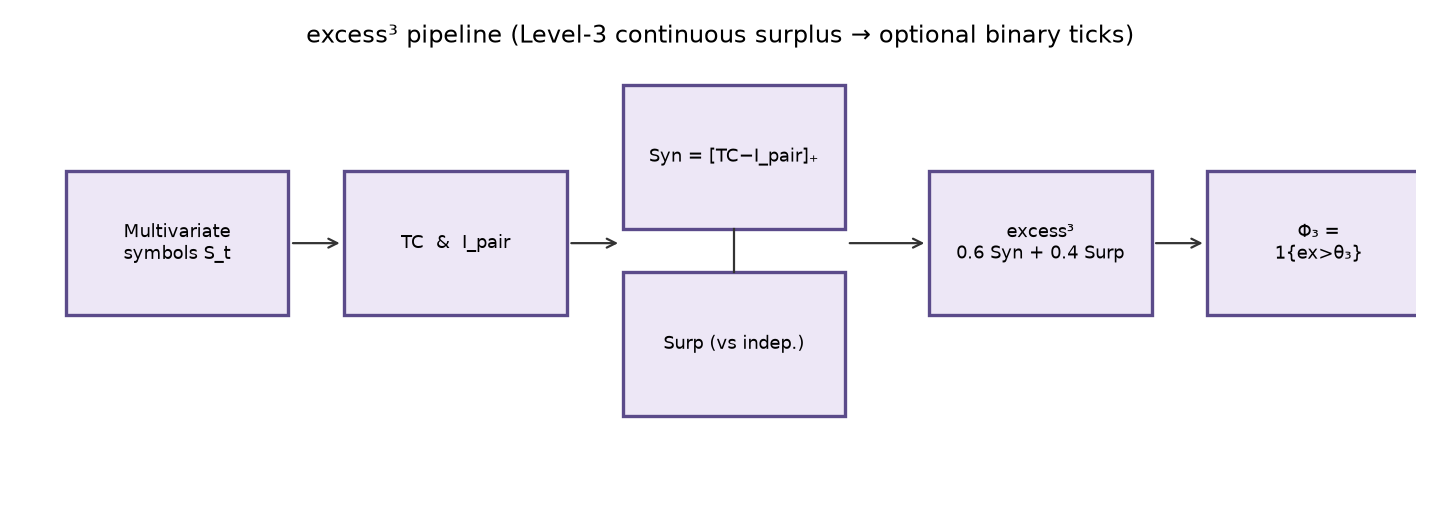
\includegraphics[width=\textwidth]{figures/fig1_schematic.png}
\caption{Map of the construction (paper overview). Multivariate series are
encoded as Bandt--Pompe ordinal symbols $S_t$; on each window one computes
total correlation (TC) and the pairwise MI baseline $I_{\mathrm{pair}}$,
forms the residual $\mathrm{Syn}=[\mathrm{TC}-I_{\mathrm{pair}}]_+$ and the
independence surprise $\mathrm{Surp}$, then the hybrid continuous surplus
$\mathrm{excess3}=0.6\,\mathrm{Syn}+0.4\,\mathrm{Surp}$. Binary
$\Phi_3=\mathbf{1}\{\mathrm{excess3}>\theta_3\}$ is an optional tick only.
Inference (Section~\ref{sec:inference}) applies phase-shuffle nulls to the
full contrast (e.g.\ $|\Delta\mathrm{excess3}|$); synthetic arms G0--G3
(Section~\ref{sec:validation}) check directional behaviour under that
contract.}
\label{fig:schematic}
\end{figure}

\subsection{Results}
\label{sec:val_results}

Table~\ref{tab:results} summarises ensemble metrics.
Figure~\ref{fig:traj} shows mean $\pm$1~SD trajectories for G0 and G1.
Figure~\ref{fig:nulls} illustrates null distributions of $\Delta$ for
example realisations. Figure~\ref{fig:sens} reports sensitivity to $w$ and
$\theta_3$. Figure~\ref{fig:binary} contrasts continuous excess$^3$ with
binary ticks on a single G1 realisation. Figure~\ref{fig:bars} summarises
effect sizes and null extremity rates across arms.

\begin{table}[H]
\centering
\caption{Ensemble results ($R=\NumR$, $B=\NumB$, reference hyperparameters).
$\mathrm{frac}_{p<0.05}$ is the fraction of realisations with two-sided
phase-shuffle $p<0.05$ on $|\Delta\mathrm{excess3}|$.}
\label{tab:results}
\begin{tabular}{@{}lrrrrrr@{}}
\toprule
Arm & mean pre & mean post & mean $\Delta$ & median $p$ & $\mathrm{frac}_{p<0.05}$ & $\Phi_3$ occ.\ post \\
\midrule
G0 & \GzeroPre & \GzeroPost & \GzeroDelta & \GzeroMedP & \GzeroFrac & \GzeroOccPost \\
G1 & \GonePre & \GonePost & \GoneDelta & \GoneMedP & \GoneFrac & \GoneOccPost \\
G2 & \GtwoPre & \GtwoPost & \GtwoDelta & \GtwoMedP & \GtwoFrac & \GtwoOccPost \\
G3 & \GthreePre & \GthreePost & \GthreeDelta & \GthreeMedP & \GthreeFrac & \GthreeOccPost \\
\bottomrule
\end{tabular}
\end{table}

\begin{figure}[H]
\centering
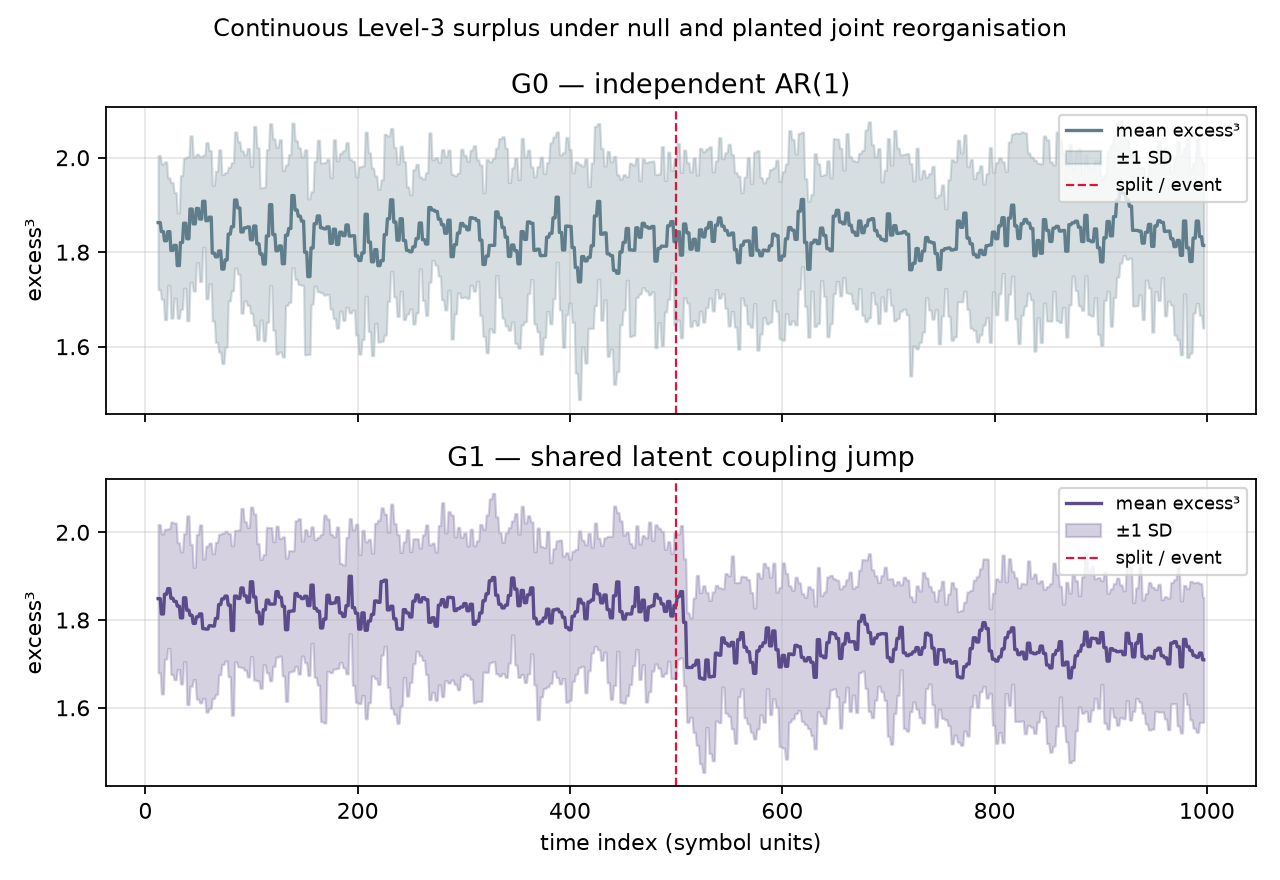
\includegraphics[width=0.95\textwidth]{figures/fig2_g0_g1_trajectories.png}
\caption{Mean excess$^3(t)$ $\pm$1~SD over realisations. Vertical line:
event/split. G0 remains flat; G1 shows a clear post-event shift after the
shared-latent coupling jump (downward under this generator; inference uses
two-sided $|\Delta|$).}
\label{fig:traj}
\end{figure}

\begin{figure}[H]
\centering
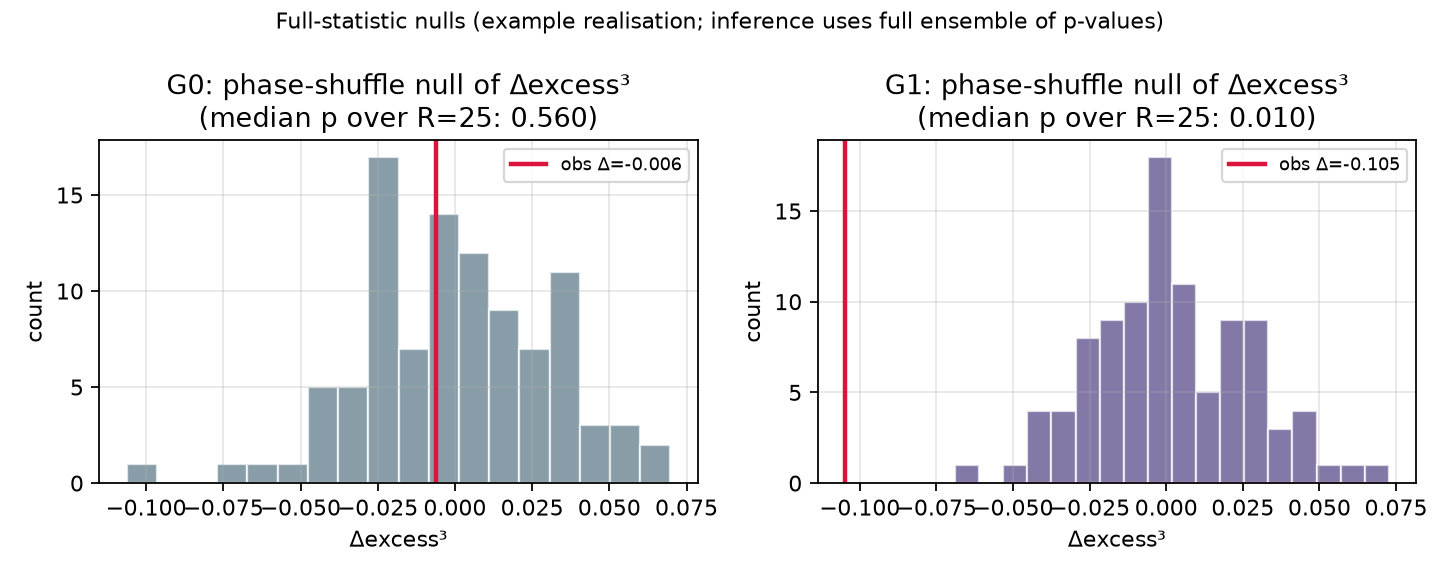
\includegraphics[width=0.95\textwidth]{figures/fig3_nulls_delta.png}
\caption{Phase-shuffle null histograms of $\Delta\mathrm{excess3}$ for an
example realisation in G0 and G1, with observed $\Delta$ marked. Ensemble
inference uses the full set of per-realisation $p$-values
(Table~\ref{tab:results}).}
\label{fig:nulls}
\end{figure}

\begin{figure}[H]
\centering
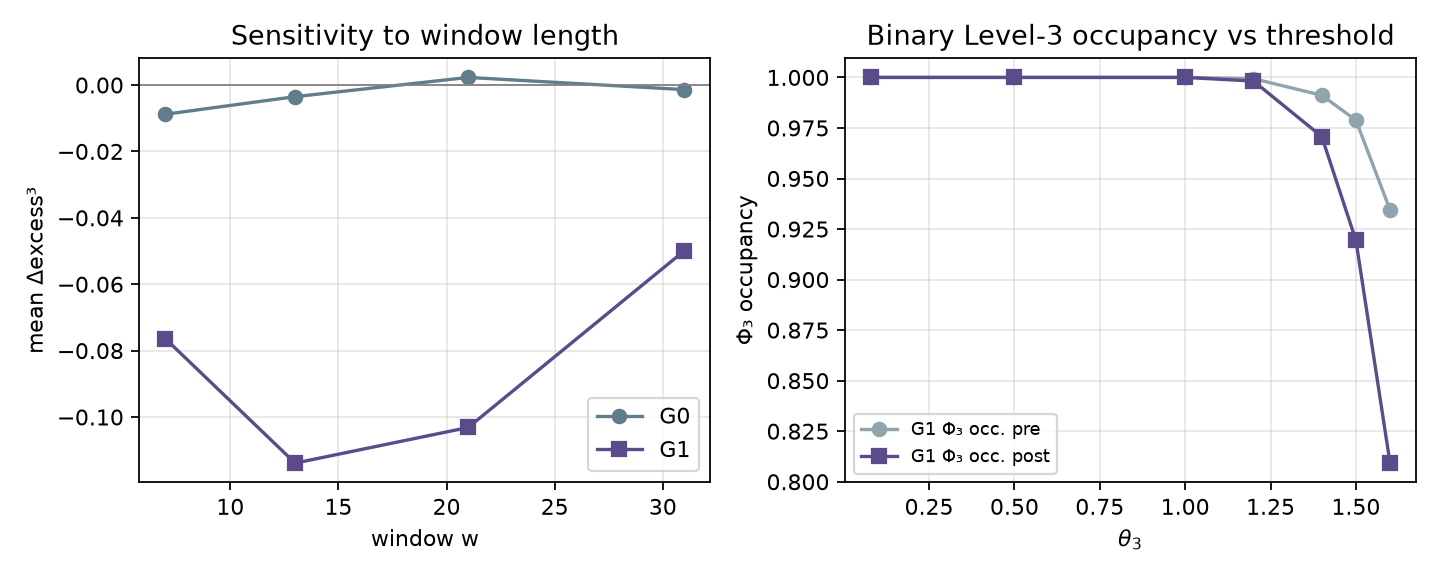
\includegraphics[width=0.95\textwidth]{figures/fig4_sensitivity.png}
\caption{Left: mean $\Delta\mathrm{excess3}$ versus window $w$ for G0 and G1
(qualitative separation stable across moderate $w$). Right: $\Phi_3$
occupancy versus $\theta_3$ on G1 (pre vs post). At the reference
$\theta_3=0.08$ (vertical dashed line) occupancy saturates; only thresholds
near the bulk of continuous excess$^3$ ($\theta_3\gtrsim 1.2$) yield
pre/post occupancy contrast---reinforcing continuous primacy under threshold
uncertainty.}
\label{fig:sens}
\end{figure}

\begin{figure}[H]
\centering
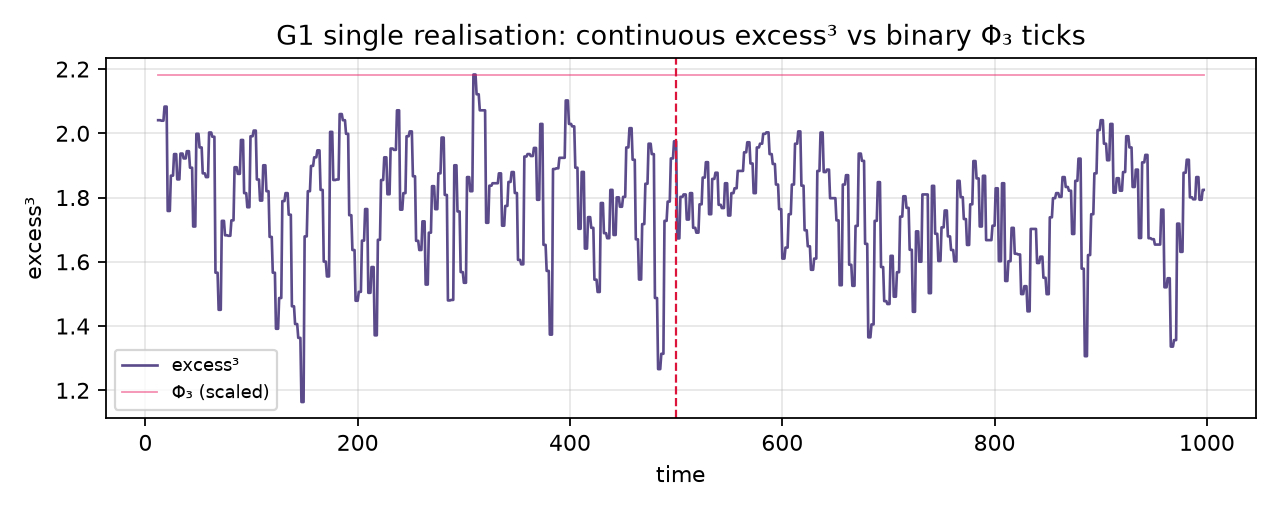
\includegraphics[width=0.92\textwidth]{figures/fig5_continuous_vs_binary.png}
\caption{Single G1 realisation: continuous excess$^3$ versus scaled
$\Phi_3$ ticks. Binary occupancy depends on $\theta_3$; continuous magnitude
carries the primary contrast.}
\label{fig:binary}
\end{figure}

\begin{figure}[H]
\centering
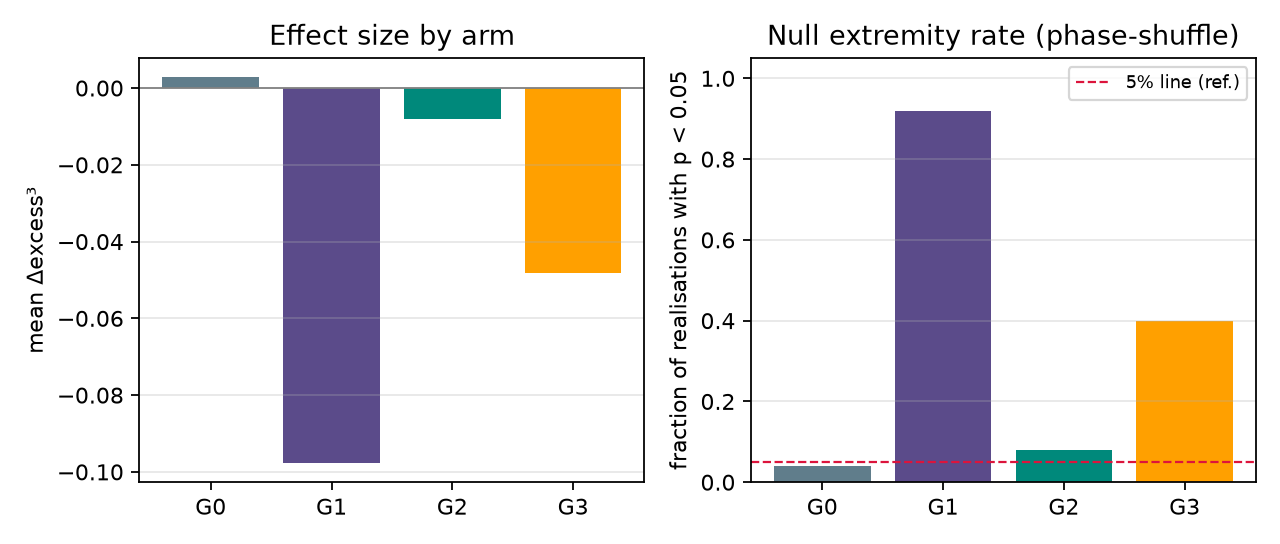
\includegraphics[width=0.92\textwidth]{figures/fig6_arm_summary.png}
\caption{Left: mean $\Delta\mathrm{excess3}$ by arm. Right: fraction of
realisations with phase-shuffle $p<0.05$.}
\label{fig:bars}
\end{figure}

\paragraph{Interpretation.}
G0 behaves as a near-null: mean $\Delta=\GzeroDelta$, median
$p=\GzeroMedP$, and only $\GzeroFrac$ of realisations with $p<0.05$
(consistent with the nominal rate under a well-calibrated null). G1
produces a clear mean shift $\Delta=\GoneDelta$ with median
$p=\GoneMedP$ and $\GoneFrac$ of realisations extreme under the
pre-specified two-sided phase-shuffle null, meeting the design success
criterion ($\ge 80\%$ with $p<0.05$). The \emph{negative} sign under the
shared-latent generator is methodologically informative rather than a
failure: stronger common coupling after the event raises pairwise MI
baselines, which can shrink the residual $\mathrm{Syn}=[\mathrm{TC}-I_{\mathrm{pair}}]_+$
even while joint structure reorganises. Inference therefore targets
$|\Delta\mathrm{excess3}|$, not a forced positive direction.
G2 (coupled logistic) is near-null in this particular design (mean
$\Delta=\GtwoDelta$, $\GtwoFrac$ extreme)---a reminder that not every
nonlinear coupling inflates excess$^3$. G3 (pairwise only) is intermediate
(mean $\Delta=\GthreeDelta$, median $p=\GthreeMedP$, $\GthreeFrac$
extreme): weaker extremity than G1 but not pure null, consistent with
partial leakage of pairwise structure into the hybrid score. Magnitudes
and signs remain generator-dependent and should not be universalised.

Sensitivity panels indicate that G0/G1 separation in
$\Delta\mathrm{excess3}$ is stable across moderate window lengths $w$.
At the reference binary threshold $\theta_3=0.08$, $\Phi_3$ occupancy is
saturated on all four arms (mean continuous excess$^3$ near $O(1)$);
raising $\theta_3$ into the bulk produces pre/post occupancy contrast on
G1, but binary tick rates then become threshold-dominated. Continuous
$\Delta\mathrm{excess3}$ remains the primary Level-3 contrast under
threshold uncertainty.

% =============================================
\section{Downstream uses}
\label{sec:downstream}

\begin{itemize}[leftmargin=*,itemsep=3pt]
  \item \textbf{High-order feature.}
  excess$^3$ or $\Delta\mathrm{excess3}$ as input to classifiers or regime
  detectors when integration/emergence proxies are of interest.
  \item \textbf{Regulariser.}
  Penalties or bonuses on order-3 synergy during model training (domain
  dependent; use with care).
  \item \textbf{Experimental contrast.}
  Pre/post or condition A/B comparisons with phase-shuffle (or design-based)
  nulls on $\Delta\mathrm{excess3}$.
  \item \textbf{Path to excess$^k$.}
  The paradigm extends to $k$-tuples; computational cost grows rapidly with
  $k$. excess$^3$ is the current expressivity--feasibility sweet spot; binary
  ticks become especially useful for $k>3$ to limit dimensionality.
\end{itemize}

% =============================================
\section{Limitations}
\label{sec:limitations}

\begin{enumerate}[leftmargin=*,itemsep=3pt]
  \item Weights and the exact pairwise baseline remain heuristic, fixed for
  falsifiability rather than optimality.
  \item Plug-in joint estimation is biased in small samples; report $T$ and
  prefer surrogate inference.
  \item excess$^3$ does not substitute for full PID when samples and
  estimators allow.
  \item Synthetic arms are minimal; they support directional claims, not a
  catalogue of all bifurcations or empirical noise structures
  \citep{Strogatz2001}.
  \item ``Integration'' language is theory-laden; the statistic measures
  high-order dependence, not a unique philosophical notion of emergence.
\end{enumerate}

% =============================================
\section{Discussion and outlook}
\label{sec:discussion}

This manuscript freezes the canonical Level-3 contract for the
Systemic Tau / RECD paradigm: a continuous, pre-specified hybrid proxy;
binary ticks as optional discretisation; phase-shuffle inference on full
contrasts; parallel nesting without hard Boolean ascent; and an explicit
non-causal, non-PID-complete reading. Section~\ref{sec:design} collects the
six fixed choices that most often generate applied confusion (weights,
Syn/Surp, continuous primacy, PID scope, nulls, nesting). Pedagogical
companions in English and Spanish may aid first contact or teaching; they
are not alternative specifications.

\subsection{Minimum reporting checklist}
\label{sec:checklist}

To reduce misuse and silent non-comparability across studies, any empirical
report that uses excess$^3$ should state at least:

\begin{enumerate}[leftmargin=*,itemsep=2pt]
  \item \textbf{Hyperparameters:} $m$, $\tau$, $w$, $\theta_3$ (if $\Phi_3$
  is shown), and stride if windows are thinned.
  \item \textbf{Weights:} confirm $(0.6,0.4)$ (or another pre-registered
  pair) were fixed \emph{a~priori}, not optimised on the scientific dataset.
  \item \textbf{Null model:} surrogate type (default: independent
  phase-shuffle) and that inference was applied to the \emph{full} contrast
  statistic (e.g.\ $\Delta\mathrm{excess3}$), not only mean-versus-mean.
  \item \textbf{Continuous vs binary:} always report continuous excess$^3$
  (trajectories and/or $\Delta$); $\Phi_3$ occupancy alone is incomplete.
  \item \textbf{Sample geometry:} $T$ (or $T_{\mathrm{eff}}$), $N$, and
  alphabet size $m!$ (joint support grows as $(m!)^N$).
\end{enumerate}

Natural extensions include: (i)~replacing Eq.~\eqref{eq:excess3} by a
stable PID synergy atom when estimators permit
\citep{Williams2010,Lizier2014}; (ii)~lagged/directed excess$^3$ for
asymmetric dependence; (iii)~excess$^k$ with cost-aware designs; (iv)~joint
reporting standards with $\tau_s$ under multi-cue RECD weighting
\citep{Padilla2026framework}. Empirical domain papers (cardiac, ecological,
neural) should cite this specification rather than re-deriving ad~hoc
Level-3 variants.

% =============================================
\section{Conclusion}
\label{sec:conclusion}

excess$^3$ is the continuous Level-3 surplus measure of the RECD hierarchy:
a pre-specified combination of synergistic residual multiinformation and
independence-model surprise on multivariate ordinal symbols. It is the
primary magnitude for order-3 irreducibility claims; $\Phi_3$ only counts
threshold crossings. Used with honest nulls and stated limitations, it
offers a practical bridge between the ideal of PID synergy and the sample
sizes of real complex systems---no more, and no less.

% =============================================
\section*{Data and code availability}

\begin{sloppypar}
Manuscript sources, figures, ensemble JSON outputs, and validation scripts
for this document family are public at
\href{\ExcessThreeRepo}{\ExcessThreeRepoShort}
(folders \texttt{methods/}, \texttt{intro/}, \texttt{primer/}).
A versioned archival DOI will be added upon Zenodo release.
Reference Level-3 code matches the open \texttt{systemictau} /
Academy Learning Tau stack \citep{Padilla2026software}
(Zenodo record \texttt{20576241}).
Reproduction of the synthetic battery needs a standard scientific Python
stack (NumPy, SciPy, and related libraries) plus the Level-3 reference
implementation on \texttt{PYTHONPATH}; see the repository README.
\end{sloppypar}

\section*{Pedagogical companions}

Optional reading that does \emph{not} redefine the statistic:
\begin{itemize}[leftmargin=*,itemsep=2pt]
  \item English cross-disciplinary guide \citep{Padilla2026primer}
  (intuition, domain vignettes, teaching notes).
  \item Spanish dense introduction with integrated synthetic figures
  \citep{Padilla2026intro}.
\end{itemize}
Cite \emph{this} methods paper for equations, null protocol, reporting
checklist, and claim-level validation.

\section*{Funding}

No dedicated external grant funded this methods preprint. The broader
Systemic Tau / RECD programme is developed as independent research.

\section*{Competing interests}

The author declares no competing interests.

\section*{License}

This preprint is intended for distribution under a Creative Commons
Attribution 4.0 International licence (CC~BY~4.0) upon public deposit,
unless a venue requires a different open licence.

\section*{Acknowledgements}

Errors of specification or exposition remain the author's.

% =============================================
\bibliographystyle{plainnat}
\bibliography{references}

% =============================================
\appendix
\section{Pseudocode (reference implementation)}
\label{app:pseudo}

\begin{verbatim}
# Windowed symbols S[t, i], i=1..N
TC  = sum_i H(S[:,i]) - H_joint(S)
Ipair = (N-1) * mean_{i<j} MI(S[:,i], S[:,j])
Syn = max(TC - Ipair, 0)

Surp = 0
for each joint tuple s with empirical p_obs:
    p_ind = product_i p_i(s_i)
    Surp += p_obs * max(log2(p_obs/p_ind), 0)

excess3 = 0.6*Syn + 0.4*Surp
Phi3    = 1 if excess3 > theta3 else 0
\end{verbatim}

\section{Reproducibility parameters}
\label{app:repro}

Reference synthetic battery (from the archival script directory):
\begin{verbatim}
python3 generate_synthetic_validation.py
# optional: fill LaTeX number macros from JSON
python3 fill_numbers_from_json.py
\end{verbatim}
\noindent Environment: Python~3 with NumPy/SciPy (and Matplotlib if
regenerating figures). Ensemble defaults match the macros in
\texttt{numbers.tex} / \texttt{validation\_results.json}
($R=\NumR$, $B=\NumB$, $T=\NumT$). Do not retune weights or the null on
the same scientific dataset used for hypothesis claims
(Section~\ref{sec:design}).
Outputs: \texttt{figures/*.png}, \texttt{notes/validation\_results.json},
\texttt{notes/validation\_summary.md}. Seeds are deterministic functions of
arm index and realisation index as coded in the script.

\end{document}
